\documentclass[border=3pt]{standalone}
\usepackage{tikz}
\usetikzlibrary{arrows.meta,calc,positioning}
\tikzset{pin/.style={-{Stealth[length=5pt]}},
  ff/.style={draw, thick, minimum width=10mm, minimum height=16mm, font=\sffamily\small},
  cloud/.style={draw, thick, rounded corners=3pt, minimum width=24mm, minimum height=13mm, font=\sffamily\small}}
\begin{document}
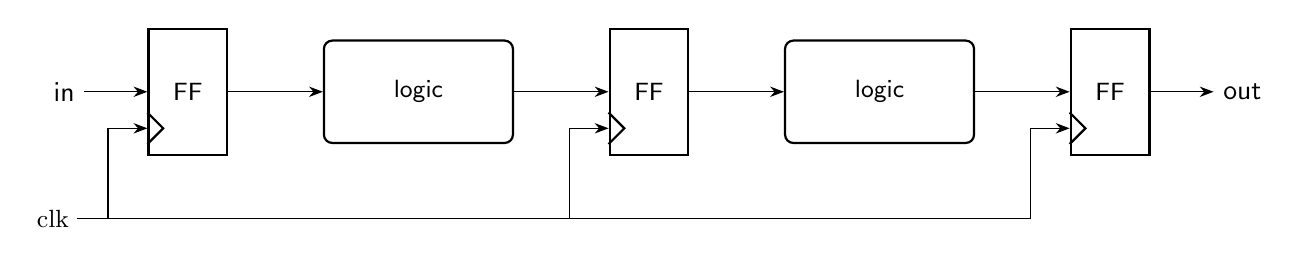
\begin{tikzpicture}[font=\sffamily, node distance=10mm]
  \node[ff] (f1) {FF};
  \node[cloud, right=12mm of f1] (a) {logic};
  \node[ff, right=12mm of a] (f2) {FF};
  \node[cloud, right=12mm of f2] (b) {logic};
  \node[ff, right=12mm of b] (f3) {FF};
  % clock triangles
  \foreach \n in {f1,f2,f3}{\draw[thick] ($(\n.south west)+(0,1.5mm)$) -- ++(2mm,2mm) -- ++(-2mm,2mm);}
  % datapath
  \draw[pin] ($(f1.west)+(-8mm,0)$) node[left]{in} -- (f1.west);
  \draw[pin] (f1.east) -- (a.west);
  \draw[pin] (a.east) -- (f2.west);
  \draw[pin] (f2.east) -- (b.west);
  \draw[pin] (b.east) -- (f3.west);
  \draw[pin] (f3.east) -- ++(8mm,0) node[right]{out};
  % clk rail below; branches rise and enter each west edge at the wedge
  \coordinate (cA) at ($(f1.south west)+(-5mm,-8mm)$);
  \coordinate (cB) at ($(f2.south west)+(-5mm,-8mm)$);
  \coordinate (cC) at ($(f3.south west)+(-5mm,-8mm)$);
  \node[font=\small] at ($(cA)+(-7mm,0)$){clk};
  \draw ($(cA)+(-4mm,0)$) -- (cC);
  \draw[pin] (cA) |- ($(f1.south west)+(0,3.5mm)$);
  \draw[pin] (cB) |- ($(f2.south west)+(0,3.5mm)$);
  \draw[pin] (cC) |- ($(f3.south west)+(0,3.5mm)$);
\end{tikzpicture}
\end{document}
